\documentclass[authordate, empirical, issue]{jote-new-article}

\usepackage{caption}

\usepackage{tabularx}

\usepackage{graphicx}

\usepackage{hyperref}

\usepackage[backend=biber,style=apa]{biblatex}


\jotetitle{"Not Again": \\When the Therapist Resists}
\footertitle{"Not Again": When the Therapist Resists}
\keywordsabstract{group music therapy, countertransference, obsessive compulsive disorder, aggression, self-reflection}
\abstracttext{This article covers the first part of a group music therapeutic process in the inpatient multidisciplinary, psychoanalytical oriented treatment of a young woman suffering an obsessive-compulsive disorder. After a description of some basic assumptions of the music therapist about risks and mistakes in a music therapeutic framework, the unfolding dynamics in the therapeutic relationship are explained. 
The combination of strong hidden emotions, unstoppable improvisations and the unspoken reaction of group members, led to a moment where the therapist actively withdrew in a musical improvisation. This particular moment is the climax of the mistake, but it also opened a new door in the therapeutic process.
Reflecting on this matter, we find the tension between the importance and the risk of countertransference and the need for supervision and discussion. Suggestions for music therapeutic interventions are made and the impact of the coping strategy and basic assumptions of the therapist are discussed.
}
\runningauthor{Fiers}
\jname{Journal of Trial \& Error}
\jyear{2023}
\paperdoi{10.36850/tva4-0m85}
\paperreceived{May 27, 2023}
\paperaccepted{September 25, 2023}
\paperpublished{November 30, 2023}
\paperpublisheddate{2023-11-30}
\author[1]{\mbox{Nele Fiers\orcid{0000-0002-8394-8598}}}
\affil[1]{Kliniek Sint-Jozef Pittem - Muze op maat}
\corremail{\href{mailto:nele.fiers@gmail.com}{nele.fiers@gmail.com}}
\corraddress{Kliniek Sint-Jozef Pittem - Muze op maat}
\runningauthor{Fiers}
\jwebsite{https://journal.trialanderror.org}
\articletype{Untangling Strings - Case Study}
\jvolume{3}
\jissue{2}
\jpages{31--38}

\specialissue{Untangling Strings -- Further Explorations of Mistakes in Music Therapy}
\begin{filecontents}{bibliography.bib}
	@book{Austin2008,
    title       = {The theory and practice of vocal psychotherapy: {S}ongs of the self},
    author      = {Austin, D.},
    publisher   = {Jessica Kingsley Publishers},
    date        = {2008}
}


@inbook{Harris2022,
    title       = {Mistakes and relational enactments},
    author      = {Harris, B. T.},
    editor      = {Gilboa, A. and Hakvoort, L.},
    publisher   = {ArtEZ Press},
    date        = {2022},
    pages       = {87--93},
    booktitle     = {Breaking strings: explorations of mistakes in music therapy}
}


@book{Johnson1991,
    title       = {Owning your own shadow},
    author      = {Johnson, R. A.},
    publisher   = {HarperCollins Publishers},
    date        = {1991}
}


@article{Miller1997,
    title       = {The drama of the gifted child: {T}he search for the true self},
    author      = {Miller, A.},
    place       = {Basis Books},
    date        = {1997}
}


@book{Ogden1989,
    title       = {The primitive edge of experience},
    author      = {Ogden, T. H.},
    publisher   = {Jason Aronson Inc},
    date        = {1989}
}
\end{filecontents}

\begin{document}
\begin{frontmatter}
  \maketitle
  \begin{abstract}
    \printabstracttext
  \end{abstract}
\end{frontmatter}


\setcounter{page}{31}

\subsection{Wrong}

“Any interpretation is by definition wrong.” This quote by one of the professors in my music psychotherapy training keeps ringing in my head. I remember myself, still in my bachelor years, being impressed and feeling warned by these words.



This statement was framed by psychoanalytical thoughts about transference and countertransference, but also by the explanation that every person has a unique, personal and time-bound reaction to music. It helped me to realize, then and today, that my reactions and opinions within and around music therapy -- no matter how many angles I try to consider -- never cover the whole picture. They might only be a small part of it. It makes me feel humble about my view about patients, their sounds and music, their reaction and mine. At the same time, it opens a wide playground for interaction and dialogue.



“Music has no meaning” was another statement. Maybe you can imagine the faces of the group of future music therapists, fearing they would study 5 years to end up with a meaningless profession. Perhaps you can also imagine the relief, hearing the nuance: “Music has no meaning in the way words do, as words are signifiers. There is no such thing as ‘a sad music' or ‘a happy music', that has the same effect on all humans.”



These are only two thoughts, but they put me on a track where I started balancing between being humble on the one hand and on the other, attaching importance to my own (counter)transference reactions while improvising, listening, singing, talking and being silent. Generalizing about music and its effect on people -- be it emotional, physical, rational -- was perceived by me as a mistake. The biggest risk seemed to be facilitating a false self with a client instead of searching for and reinforcing the true self.



This balance is an ongoing process, and part of my everyday work in a psychiatric hospital for teenagers, young adults and adults. I will come back to this topic in the reflection later in this article.



This case study describes how I, as a music therapist with about 10 years of experience, slowly get tangled in a (musical) relationship with Obi, a member of one of the music therapy groups I lead. A complex interplay of assumptions, avoidance and group dynamics leads to intense countertransference feelings and reactions, in which I as a therapist lose overview and react to Obi from a tunnel vision. We focus on the elements that lead to the mistake that has been made and on how the situation evolves after the mistake. This brings us to the reflection part that highlights the situation from different angles.







\section{Dynamics Unfolding}



\subsection{Obi}
Obi gave me permission to write about parts of her process as long as she would be anonymized, which is the case in this article. She is in her late twenties, finished high school and found a job. Recently, she got her own apartment, but is having great difficulties living there alone. Obi has been diagnosed with OCD and attends group music therapy twice a week on a residential, psychoanalytically-oriented ward of a psychiatric hospital. In this group, all patients have medium to high intellectual and verbal capacities. Obi's explorative process is combined with individual cognitive behavioural therapy, focussing on her symptoms. She has previously had a lot of treatments, but none of them offered sufficient and long-lasting results.



She expresses that she likes trying out instruments and using her voice, hoping to find a way to openly express her emotions, not really knowing what they are. Where other group members often feel inhibited to improvise, Obi can easily make a start.



When Obi says she wants to ‘express her own emotions', the spontaneity is gone. All actions she takes, are rationally directed. She thinks first what the music should be like, in what direction she wants it to go, and then she tries to translate this into sounds. It seems as if she has a framework in her head that she needs to follow. When the sounds she makes, or the music the group is playing, does not reflect her thoughts, she gets confused. When singing songs, she likes to stand next to the grand piano, singing loudly, high pitched and often in a different key than the piano accompaniment. Regarding the tempo, as long as there is a stable metre, the singing and the playing are rather parallel, but as soon as there is a slight change, or I make a musical mistake, we get lost. I wonder if she notices this: does she hear but not care, or doesn't she hear it at all? Is she aware of her musical presence or the musical presence of someone else? Anyway, for me, it feels unconnected.



It becomes clear to me that she is not used to really relating to someone or something else. It's either about merging or about staying back. Interactions in the group are rather functional or seem uncomfortable: meeting social standards. When she talks to me, I sense a mixture of Obi wanting to please and wanting to be pleased. Later in the process, it became clear that she expected others to read exactly what she was longing for. Perhaps she is not able to relate on a deeper level at this moment? Did she ever separate?



Obi experiences people as only good or only bad. I explicitly choose the word ‘experiencing', because Obi only talks in facts: ‘he is like this, she is like that'. Being bad is perceived by her as unbearable. At any point where someone makes a comment about her, or even makes a neutral observation, she is scared and is convinced she did something terrible and unforgivably wrong. This always leads to a spectacular increase of her obsessive-compulsive thoughts and behaviour.







\subsection{Playing?}



In the group improvisations, a specific kind of play appears and keeps coming back during several weeks. It is very clear that, on the one hand, she wants to play and sing her heart out and have fun, but on the other, she's tangled up by lots and lots of unspoken and unwritten rules in her mind. Underneath there is a lot of aggression, felt by staff members and other patients. Her compulsive behaviour is harmful to herself on a physical level: her skin is bleeding because of the rubbing, sometimes I see her biting very hard on her teeth or squeezing her fingers, and when she voices her thoughts they are persistent and unstoppable. What strikes me here is the strong correlation between this behaviour and some themes that come up in different therapy sessions, how quick this comes up, and how strong the reactions are. This felt aggression is not recognised by Obi herself. She considers all kinds of aggression and anger as bad. She has always been the good girl and wants to stay that way. “I am not an angry person.” “I don't know anger.” “There is no anger in me.”



Musically, her sound can be described as sharp, persistent and repetitive, going on for a long time, even when all other members of the group have already stopped playing. She is between 'holding back' and 'exploding', which makes it impossible for her to let the music evolve, to let it flow or let it go. I guess because the (effect of the) music and the playing itself does not fulfil her desires and doesn't sufficiently meet her needs, she is not able to find an ending herself. She accepts that the music stops before she gets any satisfaction. There are a lot of accents in the music. Sometimes, she changes instrument, rhythm or metre, without taking the playing of others into account. This leads sometimes to a rupture in the improvisation. The same questions with the singing come up again: is she aware of what other people are playing or not? She takes a lot of time and space, but there is never any real interpersonal connection or shared play. This provokes strong emotions in Obi, the group members and me as music therapist.







\subsection{Never enough: prelude to the/my mistake}



Some group members withdraw, or even don't start playing at all when Obi suggests doing an improvisation. Obi invites people to join but as there is no reciprocity, there is not much space for playing. The moment Obi starts playing, she is very present in a non-attuned way. When another group member is already playing in a certain tempo or movement, Obi jumps in, not noticing (or not caring?) and she starts playing in a completely different way, not consciously noticing that the other people stop playing when this happens, or that they adjust their play to her sounds, to avoid complete, ongoing chaos. Some group members get annoyed with the sounds, others are anxious, but don't say anything about this when Obi is present. Fewer and fewer group members join the improvisation with Obi.



As a music therapist, I have the feeling that I've tried everything. Playing with her, giving her space, going a bit away and coming back, joining the accents, following her sudden changes, … None of these musical interventions provoke any kind of reaction. Obi keeps on doing what she does. Only when I feed her energy, joining her need for crescendo and exploring kinds of musical ‘explosions', she uses this food and keeps on playing in the same way, only louder. However, this kind of evolution is only temporarily and stops at a certain level of energy, as if the music reaches an invisible ceiling. It is never enough and ending/stopping/quitting the improvisation is distressing for Obi.



To end an improvisation, I try playing fewer notes, doing a fade out, playing a clear cadenza (sometimes really caricatured -- how can someone NOT hear this???), making a full stop -- she keeps persisting and plays on, looking around to group members, some of them fidgeting in their chair. Sometimes, she stops after a while, sometimes I do a verbal cut: we need to end the session and/or I suggest some time for reflection. Obi stops playing, with an aggrieved and disappointed look. She has no words, but she nods immediately when I share my thought that she could keep on playing.



I notice that I am actively searching for ways to improvise with Obi, as it is never enough. Looking back on this, I realize that I never reached a state of reverie, I stayed in a state of action.



I start to get annoyed with Obi. I feel used and captured. I feel she waits for my accents or energy; it seems to be a sign and confirmation for her to play louder. I am curious where it would lead: could the music reach a kind of cathartic state? Could it bring Obi to a point where she feels satisfied? Could her aggression become undisguised? For now, this does not happen. The sharp and repetitive play keeps on going, sometimes in a medium volume, sometimes louder. We play in the same timeframe, but there is no togetherness.



I feel distressed about my position towards other group members. Some are anxious, others are frustrated, still another goes numb. I pity this situation and I feel guilty about the group when I ‘feed' Obi -not really knowing if this is the food she needs- and seeing that it leads to that much distress.



A strong countertransference reaction arises within me, and I feel split by all the reactions of the group members on Obi's way of playing.



Knowing by reports of former therapy and by literally seeing how strongly she reacts to verbal interventions towards her, these dynamics are not openly described, mentioned or questioned by the music therapist. Also the group members, who were at that time in general rather open for confrontation and discussion, remained silent.


\section{The therapist resists}



\subsection{Not again!}



Up to that point, the pattern was always the same: I evolved musically from playing with and focussing on the group to playing with and focussing on Obi. When playing with Obi, I felt not only captured as a therapist, but I also felt I was being pulled away from the group, which caused me uneasiness, guilt and powerlessness and lead to hidden anger and aggression. I really had to choose between the group and Obi, but at the same time, I had no choice but to choose Obi. Both her persistent playing and her sharp eye contact made me ‘obey' her wishes, but I also did not want or dare to leave her alone. With some hesitation, I find myself painting here the picture of a parasite on a tree.



One day, I feel, once again, the passive aggressive music coming up. Taking a picture of the situation, Obi is literally between me and the group. We share the piano, but don't share the music (see Figure 1).



\begin{figure}

  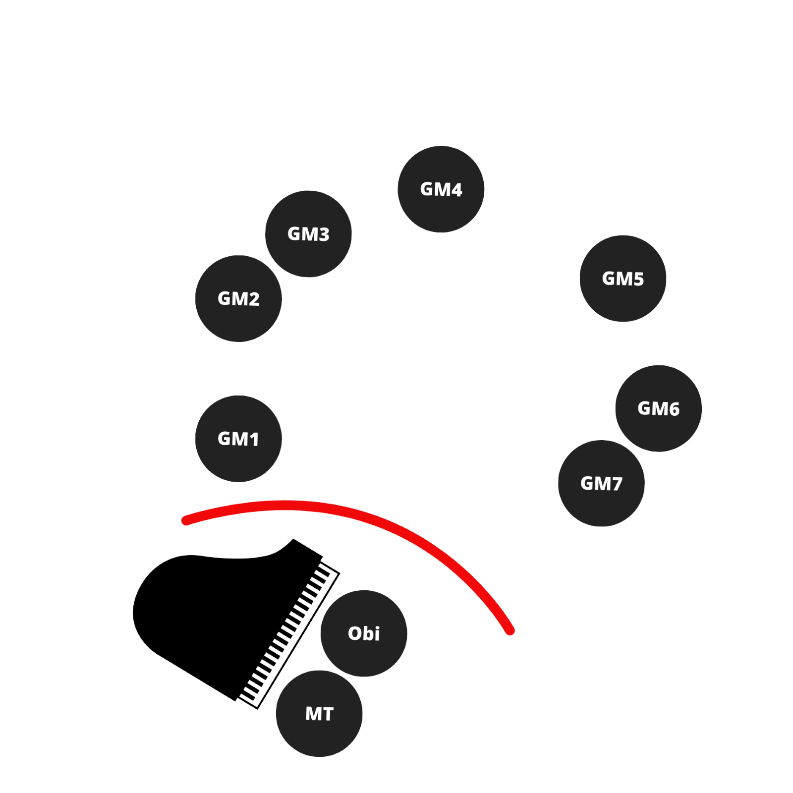
\includegraphics[width=\linewidth]{media/image1.png}

  \caption{}

  \label{fig:rId5}


\end{figure}



This time, experiencing this big gap separating the group, I actively hold back from going with Obi, staying musically away from what she is playing. I can feel her pulling me, waiting for me to join her, to feed her, but I resist. “Not again.” A musical tug-of-war. I brace myself in nearly a physical way. (See Figure 2) In the improvisation itself I was aware of the fact that I did not want to be dragged into her playing but could not/did not change this. In a way, I am aware of the group, as if I want to prove both for myself and for the group members that I can resist the suction power of Obi. The reactions in the group, the anxiety, frustration and numbness, activate a part of me to show that the situation could evolve in another direction. In the music itself, I am not connected to anyone in the room, I can only hold on to the piano and try to play something that is not for Obi.



\begin{figure}


  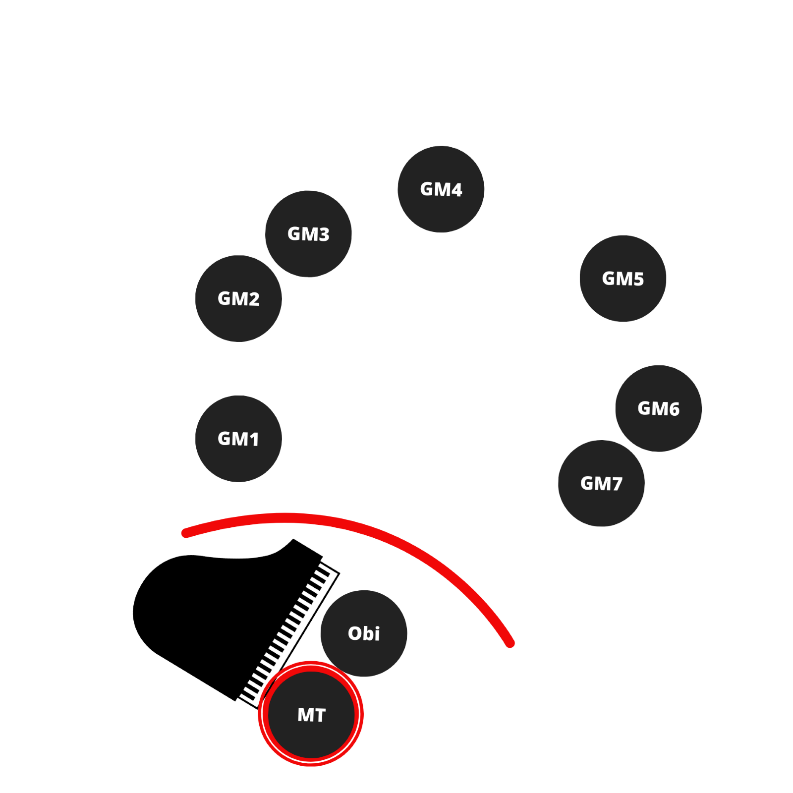
\includegraphics[width=\linewidth]{media/image2.png}

  \caption{}

  \label{fig:rId6}


\end{figure}



This holding back could have been a therapeutic decision, like I had tried before: musically playing with distance. But, in this moment, it was nothing more than a complex emotional reaction from myself: not wanting to be dragged into it once again, not wanting to leave the group alone for another ‘as if' playing time that ‘leads nowhere'. Honestly, I can see now that I was also not playing with the group; all my energy went into defensively drawing boundaries.







\subsection{Puzzled and ashamed}



{\emph{Obi is very puzzled afterwards and, seeing her like this, I come back to a reflective and mentalising state of mind. I read loneliness or sadness in her eyes. She clearly experienced something she did not understand, and I feel pity for her. It is the first time that something deep inside me resonates in contact with Obi. I am puzzled too, and in this session, I don't know how to start to verbalize.}}

{\emph{After the session I feel deeply ashamed to have taken away a chance for therapeutic growth from her, having left her alone and resisting her musical question, not only by not reaching out to her in this improvisation, but also by avoiding earlier on to address this situation verbally. If she is really a parasite, I should have known that a parasite needs a vivid organism to survive. I don't understand how it could have come so far. Now I was the one acting passively aggressive. }}




\subsection{Contact}



The day after this session, I feel that something is changed within myself: I do not feel so annoyed anymore, I have got in touch with a strong sense of loneliness and helplessness within Obi. I feel relieved and freer. Seeing her the day before like that, I was deeply touched. I could feel her pain and a new way to make connection emerged.



I feel the urge for honesty, for breaking the silence, and I start to communicate in a gentle way, sharing some observations with her. It is the first time I feel I can talk or dare to talk. Moreover, and more important, I am more connected to myself and experience that I can fully relate to her, feeling the warmth and kindness I recognize in my work in general. In this moment, I have the impression Obi tries to listen and capture what I am saying, also visually checking my (re)action. She does not respond with words, but nods. It is not necessarily a confirming nod, but rather a nod as a sign she can take it.


\section{Conclusion}

\subsection{Reflection}



Looking back on this part of the process, I will summarize what might have been missed opportunities on the level of the music, (counter)transference and team. These reflections might be helpful to prevent similar reactions in future situations. Mistakes are inherent in therapeutic processes, but I strongly believe that we have the responsibility to reflect about them, to avoid blind and motionless repetition, like the seemingly endless repetition of the way I was musically responding to Obi.

\begin{itemize}


  \item First, I did not reflect enough on this matter with my team members or supervisor. At the time this process started, there were big organisational changes within the hospital. There was a lot of distress about this and there was not much mental space left to discuss patient issues between therapy sessions. There was no organised intervision and my own supervision was focused on another part of my work. In this regard, we can discuss what was the biggest mistake: the way things evolved in the sessions or the fact that they were not discussed in supervision. Harris (2022) describes the importance of mistakes and enactments in a music psychotherapeutic relationship, but at the other hand, Miller (1997) warns not to project unsolved themes or dynamics on the patient. This is, and will always be, a tightrope walk.Another suggestion that came up in a discussion with a colleague in the writing process of this article, was to frame the actions of Obi in the autistic-contiguous mode of Ogden (1989). Reading more about this mode and the vulnerability it implies, offered me a broader view on the situation and more compassion to Obi.



  \item
        In a way, I underestimated the severity of this dynamic. I knew how bad Obi's OCD reactions were and was (too) careful about this, but I was not aware of how this could come alive in interaction. Writing this down, I can hardly believe how I overlooked it. Why did this happen? The explanation can partly be found in a cocktail of my own coping style and transference reactions. I experienced a strong helpless feeling when I saw Obi at the beginning of her treatment being lost in her obsessive-compulsive thoughts. This clashed with how annoyed I became when seeing Obi taking so much space away from the group, seeing group members vanish and being afraid of the sharp sounds while avoiding any kind of confrontation with Obi. A parallel process in letting Obi attend both individual and group sessions might have opened the opportunity to really see her without being split by the responsibility for both the group and Obi.



  \item Clearly, my coping strategy in this situation was avoidance. I was avoiding the confrontation, and thus avoiding making mistakes. At that time in the process, it felt wrong to me to take the risk to confronting her, which might trigger OCD reactions, hopelessness and even suicidality. Not surprisingly, exactly this style leads to mistakes... In both my personal process as in supervision, this theme is brought up, and I need to keep paying attention to this matter. At the same time, it was not a coincidence that I was avoiding, as Obi was avoiding too. Austin (2008) describes both the importance and the risk of ‘the therapist's hook', an overlap of wounds of both therapist and client, causing countertransference reactions. What surprises me is that I forgot about one of my sources of inspiration: working with the concept of the shadow (Johnson, 1991). This shadow work in particular - putting emphasis on the importance of exploring and integrating split off and unwanted parts - is normally a resource for me to not avoid.



  \item
        While improvising, but also now as I look back on the process, I feel I used all musical parameters I could to find connection with Obi. What I overlooked was the possibility to install structured play forms for the whole group, so not clearly directed to Obi. Like this, we would not always have done free improvisation. It could have been interesting to observe what would have happened there, whether the opportunity for another kind of playing emerged, or whether differentiating and verbalising might have helped. I guess I was dragged too far into the situation to find a kind of meta perspective, to take some steps back and find a clearer view on the situation.



  \item Coming back to my first thoughts about making mistakes and the risk of facilitating a false self instead of reinforcing the true self, I can see that these thoughts installed in an unconscious way an imbalance in myself. I did have conscious thoughts about not being too direct to Obi, not in commenting and not in giving advice, because she took everything directly in, trying to adjust to others. Voicing that ‘student' part of myself: “I have to avoid putting her in a new musical framework, where she only takes over the wishes of the therapist or the group. This would mean she develops a new version of a false self instead of finding a way to the true self. I have to give her possibilities to explore.” But this part of me, the avoiding making mistakes as a therapist, was yelling too hard in my ears. I left her alone for too long in a no-man's-land by staying so close to my first impressions as a student. Also here, I should take more time to reflect and give myself the chance to restructure and reframe my thoughts - to dare to confront my certainties. While writing it is quite easy to do so, but the challenge is to work this out in a live-on-stage situation where there is a group, group dynamics and lots of (counter) transference.


\end{itemize}





\subsection{Becoming}

Obi had a long and difficult treatment. Sometimes the sharpness came back, sometimes I felt captured again. Writing this article helped me to keep on breathing and to stay with her throughout her struggle. Perhaps this is my final conclusion: I need to write more when processes are getting tough. Writing takes time, but it helps to get the picture clearer.







In the beginning of this music therapeutic process, I followed Obi to the piano when she went to the instrument. If I didn't, she would look at me, waiting for me to come and sit next to her. A silent rule.



After the situation I described here, I started to verbalise: “Do you want me to join you?”. Sometimes I did not play the piano and told her she could try out the whole range of the piano, while I would accompany, for example, on guitar.



I smiled the first time she asked me if I wanted to join her. In that moment, the pressure left the room and made space for some shared experiences. We could relate to each other in an open and playful way. A milestone, a symbol of future opportunities and further growth.







\subsection{To Obi}

{\emph{Obi, you felt alone, different and strange for such a long time. I wish you satisfying, joyful and inspiring shared moments in your life. Thank you!}}


























\section{References}







\hspace*{\parindent}Austin, D. (2008) \emph{The theory and practice of vocal psychotherapy: Songs of the self.} Jessica Kingsley Publishers



Harris, B. T. (2022) Mistakes and relational enactments. In A. Gilboa \& L. Hakvoort (Eds.) \emph{Breaking strings: explorations of mistakes in music therapy} (pp. 87-93)\emph{. }ArtEZ Press



Johnson, R. A. (1991) \emph{Owning your own shadow. }HarperCollins Publishers



Miller, A. (1997) \emph{The drama of the gifted child: The search for the true self }(3\textsuperscript{rd} ed.).\emph{ }Basis Books



Ogden, T.H. (1989) \emph{The primitive edge of experience. }Jason Aronson Inc.














\end{document}